\problemname{Armrests}

The Petitess Organization (PO) is having a meeting and the $N$ members are sitting on
chairs in a ring, facing inward. Between each pair of chairs there is an armrest that at most one person can use. Each person has a preference for which arm or arms they want to place on the armrests:
\begin{itemize}
\item \texttt{V}: left arm
\item \texttt{H}: right arm
\item \texttt{A}: either left or right arm
\item \texttt{B}: both arms
\item \texttt{I}: no arm
\end{itemize}

PO is about to have a meeting and wants as many members as possible to have their preference fulfilled. Given a string describing all $N$ members' preferences, calculate the maximum number of people who can be satisfied.

\section*{Input}
On the first line is an integer $N$ ($5\le N \le 30$), the number of people in the ring. On the second line are the people's preferences, given in the order
the people are sitting, {\em counterclockwise} in the ring, as a
string consisting of $N$ letters, each being \texttt{V}, \texttt{H},
\texttt{A}, \texttt{B}, or \texttt{I}. 

\section*{Output}
Output one integer: the maximum number of people who can have their preference fulfilled.

\begin{figure}[!htb]
\begin{center}
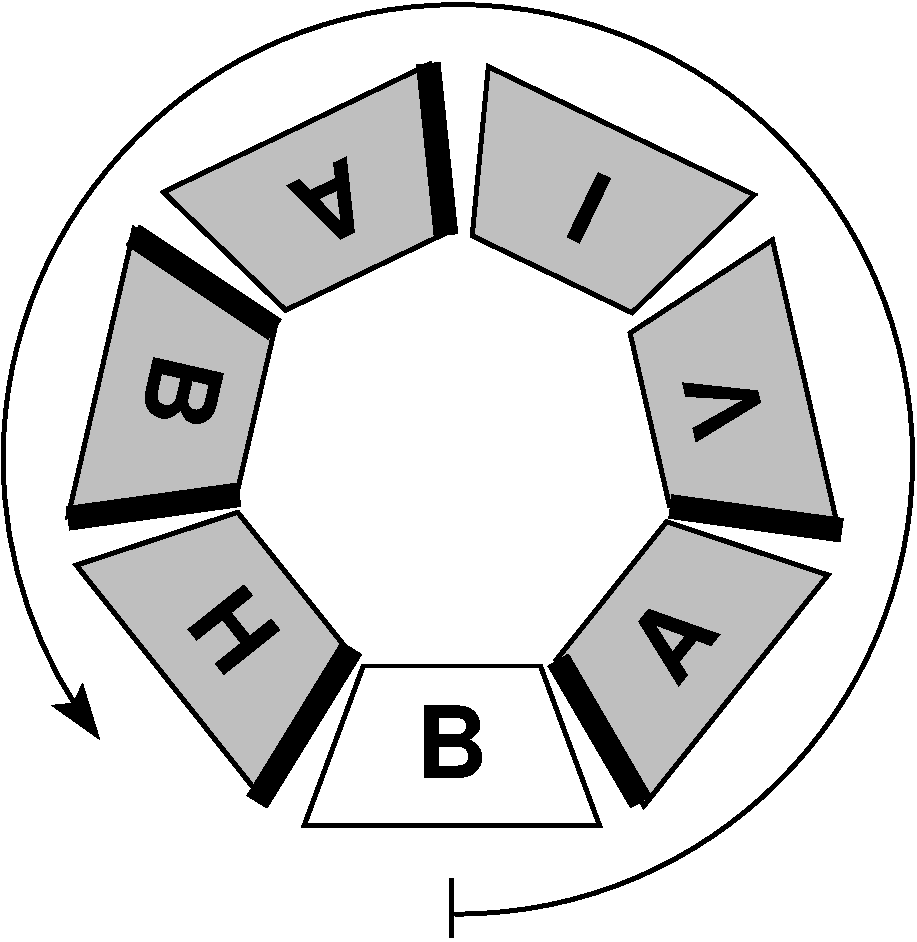
\includegraphics[width=5cm]{armstodbild.pdf}
\end{center}
\caption{The figure shows the solution to sample $1$. The thick lines indicate
arms that people have placed on the armrests. The gray color shows who has had their preferences fulfilled. The arrow marks where the given
input string starts and ends.}
\end{figure}

\section*{Scoring}
Your solution will be tested on a set of test groups.
To earn points for a group, you must pass all test cases in that group.
\noindent
\begin{tabular}{| l | l | l |}
\hline
  Group & Points & Constraints \\ \hline
  $1$    & $20$       &  $N=5$ and the first letter is \texttt{I}.\\ \hline 
  $2$    & $40$       &  $5\le N\le 15$. \\ \hline 
  $3$    & $20$       &  The first letter is \texttt{I}.\\ \hline 
  $4$    & $20$       &  No additional constraints. \\ \hline
\end{tabular}
